\documentclass[tikz,border=3pt]{standalone}
\usepackage{amsmath,amssymb}\usepackage{mathptmx}
\usepackage{tikz}
\usetikzlibrary{arrows.meta,positioning,fit,backgrounds,calc,shapes.geometric,decorations.pathreplacing}
\definecolor{ink}{HTML}{1F1F1E}
\definecolor{muted}{HTML}{5F5E58}
\definecolor{base}{HTML}{F3F3F1}
\definecolor{baseedge}{HTML}{8A8980}
\definecolor{newc}{HTML}{CDE2FB}
\definecolor{newedge}{HTML}{1C5CAB}
\definecolor{accent}{HTML}{EB6834}
\definecolor{accentlt}{HTML}{FBE1D6}
\tikzset{
  >={Stealth[length=2.2mm]},
  blk/.style={draw=baseedge, fill=base, rounded corners=2pt, align=center, font=\footnotesize,
              minimum height=10mm, inner sep=3pt, line width=0.5pt},
  newblk/.style={blk, draw=newedge, fill=newc, line width=0.8pt},
  accblk/.style={blk, draw=accent, fill=accentlt, line width=0.8pt},
  flow/.style={->, draw=ink, line width=0.6pt},
  newflow/.style={->, draw=newedge, line width=0.8pt, dashed},
  lbl/.style={font=\scriptsize, text=muted, align=center},
}

\begin{document}
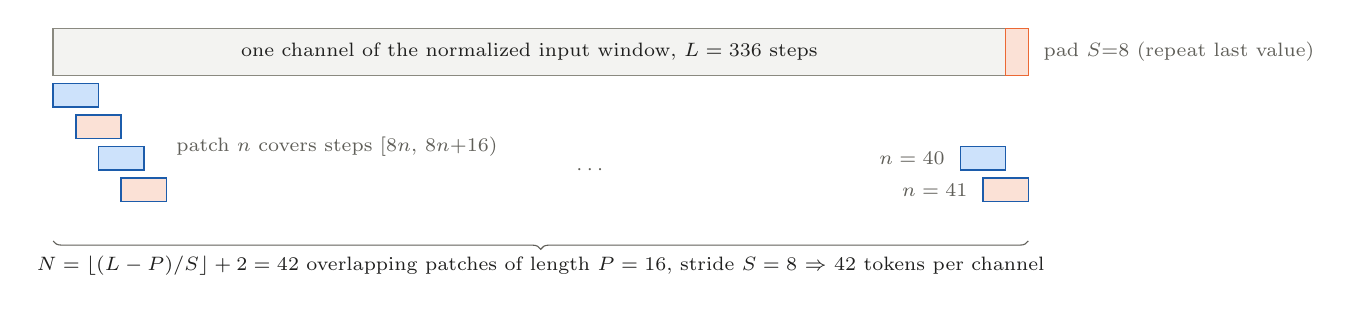
\begin{tikzpicture}[x=0.36mm, y=1mm]
  % the series line (schematic, 336 steps + 8 padded)
  \draw[line width=0.5pt, draw=baseedge, fill=base] (0,0) rectangle (336,6);
  \node[lbl, text=ink] at (168,3) {one channel of the normalized input window, $L=336$ steps};
  \draw[line width=0.5pt, draw=accent, fill=accentlt] (336,0) rectangle (344,6);
  \node[lbl, anchor=west] at (346,3) {pad $S{=}8$ (repeat last value)};
  % patches
  \foreach \i/\c in {0/newc,1/accentlt,2/newc,3/accentlt}{
    \pgfmathsetmacro{\s}{8*\i}
    \pgfmathsetmacro{\yy}{-4-4*\i}
    \draw[draw=newedge, fill=\c, line width=0.5pt] (\s,\yy) rectangle ++(16,3);
  }
  \node[lbl, anchor=west] at (40,-9) {patch $n$ covers steps $[8n,\,8n{+}16)$};
  \node[lbl] at (190,-12) {$\cdots$};
  \foreach \i/\c in {40/newc,41/accentlt}{
    \pgfmathsetmacro{\s}{8*\i}
    \pgfmathsetmacro{\yy}{-4-4*(\i-38)}
    \draw[draw=newedge, fill=\c, line width=0.5pt] (\s,\yy) rectangle ++(16,3);
  }
  \node[lbl, anchor=east] at (318,-10.5) {$n=40$};
  \node[lbl, anchor=east] at (326,-14.5) {$n=41$};
  \draw[decorate, decoration={brace, mirror, amplitude=3pt}, draw=muted] (0,-21) -- (344,-21)
     node[midway, below=2pt, lbl, text=ink] {$N=\lfloor (L-P)/S\rfloor+2=42$ overlapping patches of length $P=16$, stride $S=8$ $\Rightarrow$ $42$ tokens per channel};
\end{tikzpicture}
\end{document}
